% !TEX encoding = UTF-8
% !TEX program = pdflatex
% !TEX spellcheck = it_IT

\documentclass[a4paper, 11pt]{article}

% sintassi
\usepackage[T1]{fontenc}
\usepackage[utf8]{inputenc}
\usepackage[english]{babel}
\DeclareUnicodeCharacter{00A0}{~}
\usepackage{fullpage}
\usepackage[cochineal]{newtxmath}
\usepackage{crimson,verbatim}
\usepackage{textcomp}
\usepackage{color,soul,hyperref,mwe}

% matematica e chimica

\usepackage{siunitx,amsmath,bm,chemfig}
\newcommand{\ud}{\mathop{}\!\mathrm{d}}
\sisetup{detect-all,math-rm = \ensuremath}

\setatomsep{2em}

\newcommand\setpolymerdelim[2]{\def\delimleft{#1}\def\delimright{#2}} 
\def\makebraces[#1,#2]#3#4#5{% 
\edef\delimhalfdim{\the\dimexpr(#1+#2)/2}% 
\edef\delimvshift{\the\dimexpr(#1-#2)/2}% 
\chemmove{% 
\node[at=(#4),yshift=(\delimvshift)] {$\left\delimleft\vrule height\delimhalfdim depth\delimhalfdim 
width0pt\right.$};% 
\node[at=(#5),yshift=(\delimvshift)] 
{$\left.\vrule height\delimhalfdim depth\delimhalfdim 
width0pt\right\delimright_{\rlap{$\scriptstyle#3$}}$};}} 
\setpolymerdelim()

% tabelle e grafica
\usepackage{booktabs,graphicx,subfig,caption,pdfpages}
\captionsetup{font=small,
	format=hang,
	justification=centering,
	singlelinecheck=true,
	labelfont={sf,bf}	
}
\usepackage{float}
\floatstyle{plaintop}
\restylefloat{table}
\usepackage{multirow}
\usepackage{fancyhdr}
\pagestyle{fancy}
\fancyhead[LE,RO]{\textsl{\rightmark}}
\fancyhead[LO,RE]{\nouppercase{\leftmark}}
\fancyfoot[C]{\thepage}
\usepackage[margin=1in,headsep=.3in]{geometry}
\usepackage[suftesi]{frontespizio}
\usepackage{xparse}

\newenvironment{chapterabstract}{%
  \par\nobreak\noindent
  \textbf{\textit{Abstract}\hrulefill}\par\nobreak
  %\small
  \noindent\ignorespaces
}{%
  \par\nobreak\normalsize
  \vskip-\ht\strutbox\noindent
  \textbf{\hrulefill}%
}
\makeatletter
\NewDocumentCommand\headerspdf{ O {pages=-} m }{% [options for include pdf]{filename.pdf}
  \includepdf[%
    #1,
    pagecommand={\thispagestyle{fancy}},
    scale=1,
    ]{#2}}
\NewDocumentCommand\secpdf{somO{1}m}{% [short title]{section title}[page specification]{filename.pdf} --- possibly starred
  \clearpage
  \thispagestyle{fancy}%
  \includepdf[%
    pages=#4,
    pagecommand={%
      \IfBooleanTF{#1}{%
        \section*{#3}}{%
        \IfNoValueTF{#2}{%
          \section{#3}}{%
          \section[#2]{#3}}}},
    scale=.65,
    ]%
    {#5}}
\makeatother

\begin{document}

\section{Experimental activity}

Four  experiments have been carried out: 
\begin{enumerate}
\item Shore hardness;
\item Vicat test;
\item Melt Flow Index analysis;
\item Limiting Oxygen Index (LOI) test.
\end{enumerate}

\subsection{Shore hardness}

Shore Hardness scales are used to compare the behaviour of different materials under load. The durometer ATS FAAR has been used.
Two different scales have been employed:
\begin{itemize}
\item Shore A: presents a conical indentor and the weight applied is about 0.488 Kg. It is used for soft and flexible materials.

\item Shore D: presents a sharp indentor and the weight applied is about 3.964 Kg. It is used for hard and semi-rigid materials.

\end{itemize}

Different polymeric speciements have been tested: for each, three mesurements has been carried out with a waiting time of three seconds.

The polymers analyzed are reported in the following table\ref{tab:polymers}:


\begin{table}[htp]
	\centering
	$
	\begin{array}{ccc}
	\toprule
	\textbf{number} & \textbf{sample} & \textbf{type} \\
	\midrule
	1,24 & \text{PP + GF} & \text{thermoplastic}\\
	2 & \text{POM} & \text{thermoplastic}\\
	3 & \text{PA 11} & \text{thermoplastic}\\
	4 & \text{PE} & \text{thermoplastic}\\
	5 & \text{PVC} & \text{thermoplastic}\\
	6 & \text{PMMA + BaSO} & \text{thermoplastic}\\
	7 & \text{PBT} & \text{thermoplastic}\\
	8,9 & \text{EPDM} & \text{elastomer}\\
    10 & \text{PC} & \text{thermoplastic}\\
	11 & \text{PMMA} & \text{thermoplastic}\\
	12 & \text{generic rubber} & \text{elastomer}\\
	13 & \text{PA 6} & \text{thermoplastic}\\
	14,18,20,25,27 & \text{PU} & \text{thermoset}\\
	15 & \text{Polysilicone} & \text{elastomer}\\
	16 & \text{ABS} & \text{thermoplastic}\\
	17 & \text{PSA} & \text{thermoplastic}\\
	19 & \text{PP} & \text{thermoplastic}\\
	21 & \text{PTFE} & \text{thermoplastic}\\
	22 & \text{COC} & \text{thermoplastic}\\
	23 & \text{PA} & \text{thermoplastic}\\
	26 & \text{PET} & \text{thermoplastic}\\
	\bottomrule
	\end{array}
	$
	\caption{polymers}
	\label{tab:Polymers}
\end{table}


\begin{figure}[htp]
	\centering
	{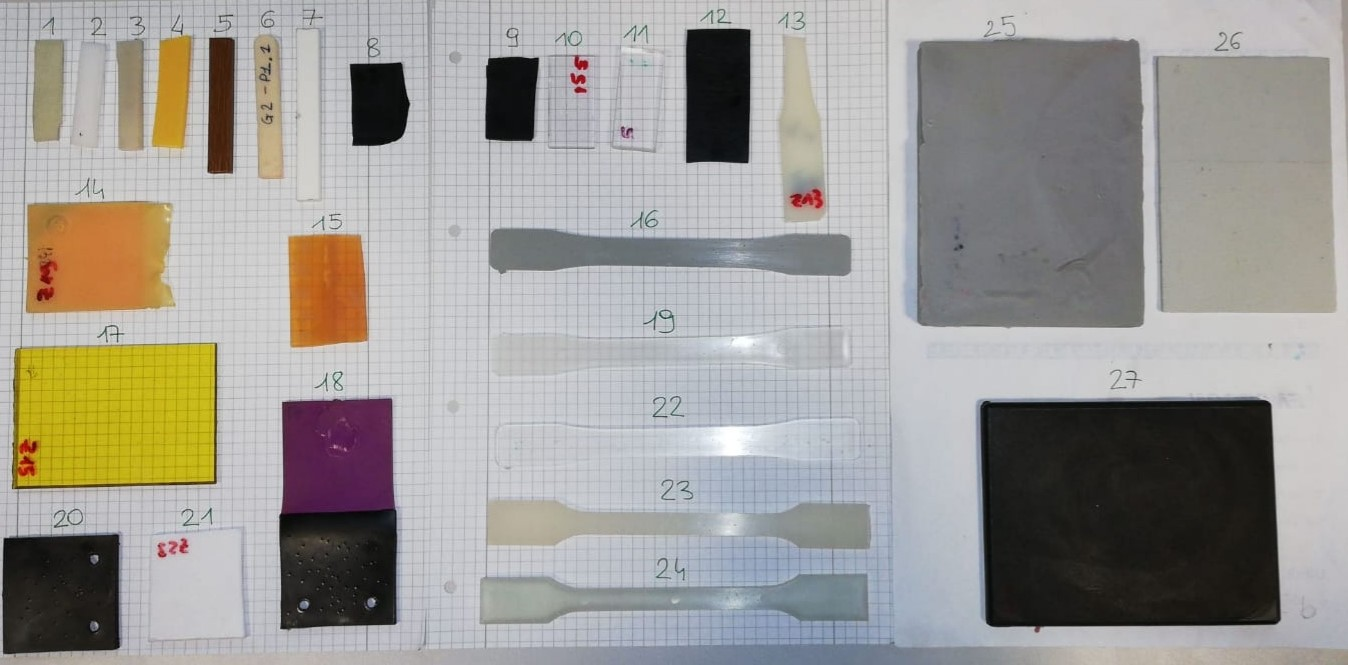
\includegraphics[scale=0.5]{materials}}
	\captionsetup{justification=centering}
	\caption{Polymers}
	\label{fig:materials}
\end{figure}

\subsection{Vicat test}

The test has been carried out in two configurations:

\begin{itemize}

\item $120$ $^\circ$ C/h, $10$ N;

\item $120$ $^\circ$ C/h, $50$ N.

\end{itemize}

The instrument used is VICAT TESTER model MP/$3$.\\
Polymers analyzed are: PC, ABS, PP. Samples lenghtxwidth is $1$x$1$ cm and the height has to be higher than the maximum penetration depth.\\
Vicat temperarature ($T_{Vicat}$) is the temperature at which the penetration is about $1$ mm.\\

\subsection{Limiting Oxygen Index}

This test allows to predict the behaviour of polymers when they are exposed to the flame. Air is blowed in the working column and the amount of oxygen is carefully modulated (its value has been taken around 21$\%$). Specimens are exposed to the flame for three minutes. The polymers analized are: PE, PP, PC, ABS. The instrument used is CEAST (ITALY) OXYGEN INDEX.

\section{Results}

\subsection{Shore hardness}

The results of the experiment are reported in figure \ref{fig:duro}:

\begin{figure}[htp]
	\centering
	{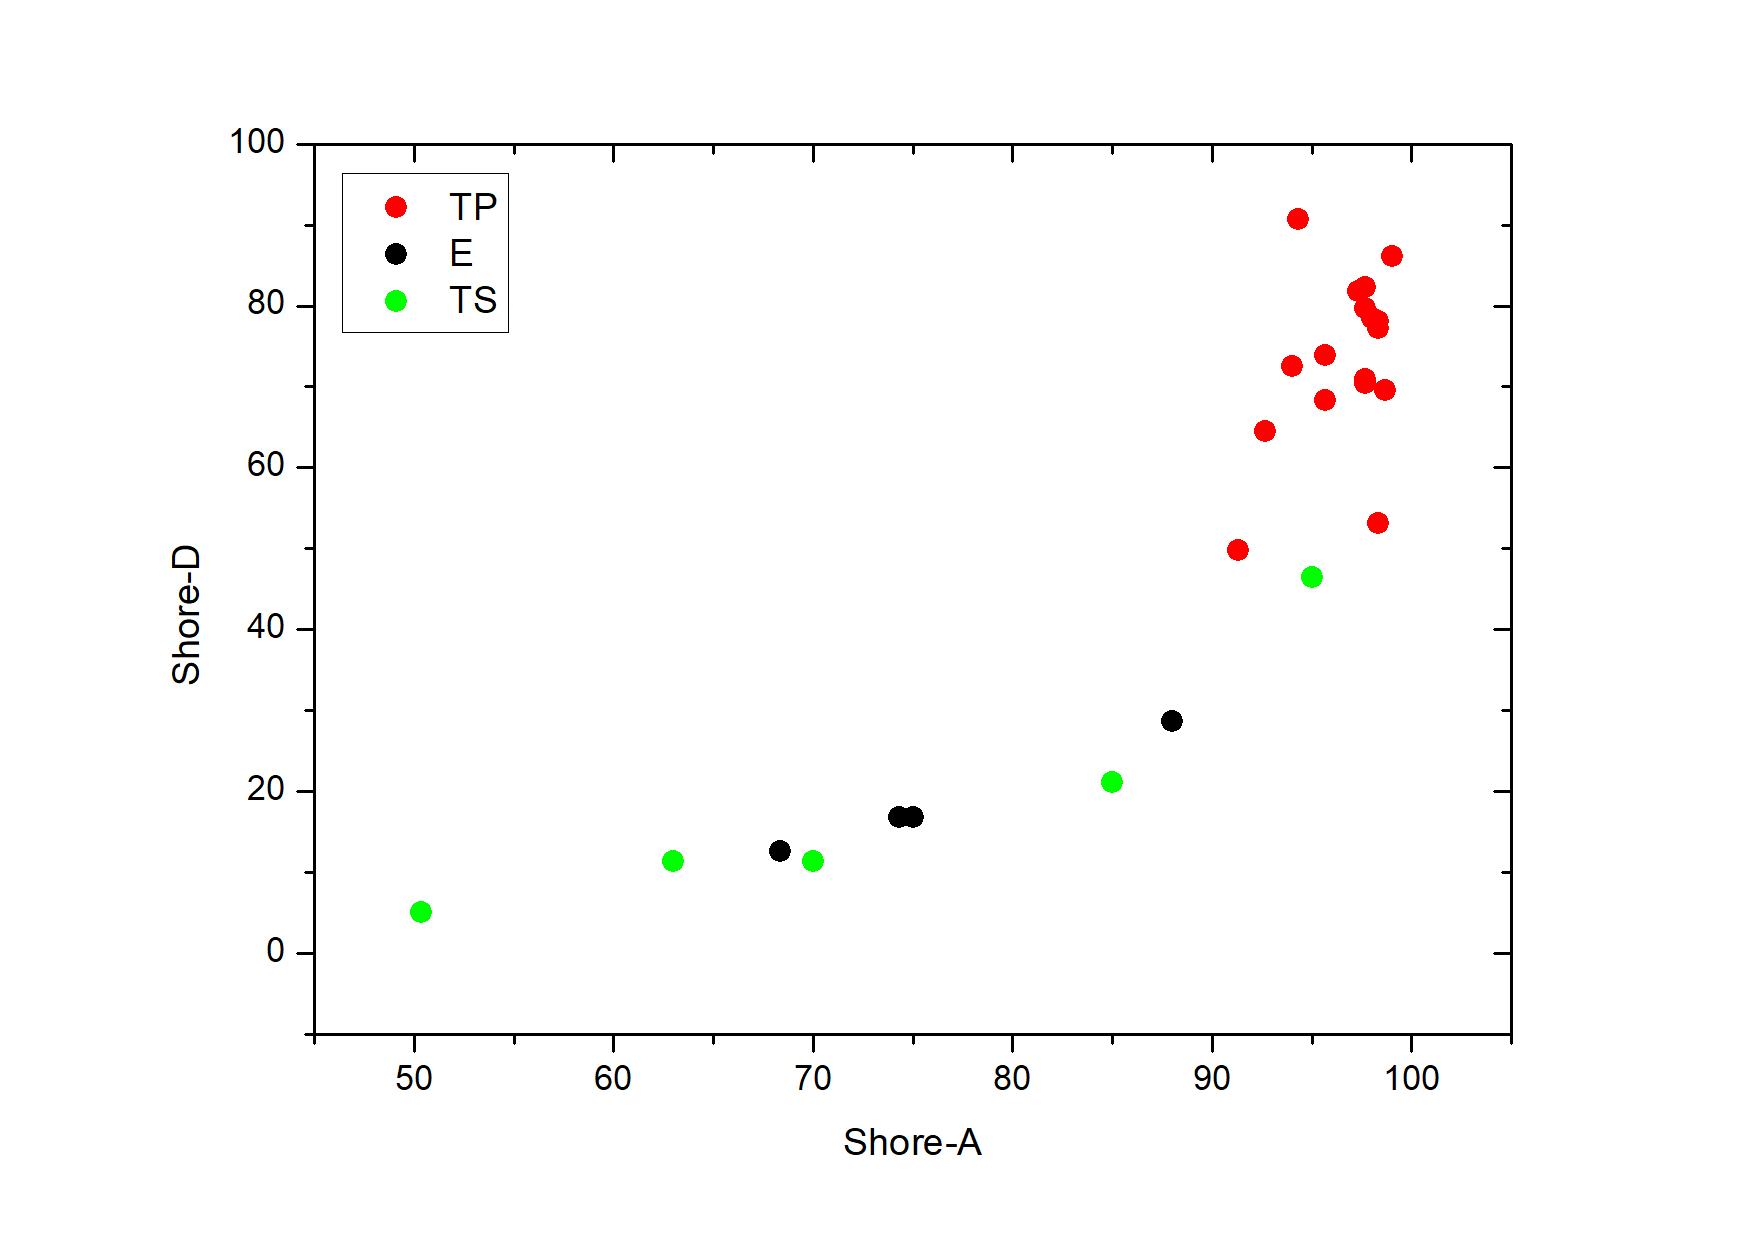
\includegraphics[scale=0.5]{duro}}
	\captionsetup{justification=centering}
	\caption{Hardness values comparison}
	\label{fig:duro}
\end{figure}

From the figure it is possible to recognize the different families of polymers (thermoplastic, elastomer, thermoset).\\
Thermoplastic polymers show the highest hardness.\\
Moreover it is possible to verify that Shore-A is more suitable for soft materials, while Shore-D for hard ones. In fact, Shore-D shows a limited dispersion of results in respect of Shore-A for materials with lower hardness.\\
The only thermoset polymer analized was polyurethane (PU). Its particular characteristic is to have a wide range of hardness (Shore-A), from 50 to 95.

\subsection{Vicat test}

The results of the penetration test are reported in the following Figures \ref{fig:vicat} - a,b.

\begin{figure}[htp]
	\centering
	\subfloat[][]
	{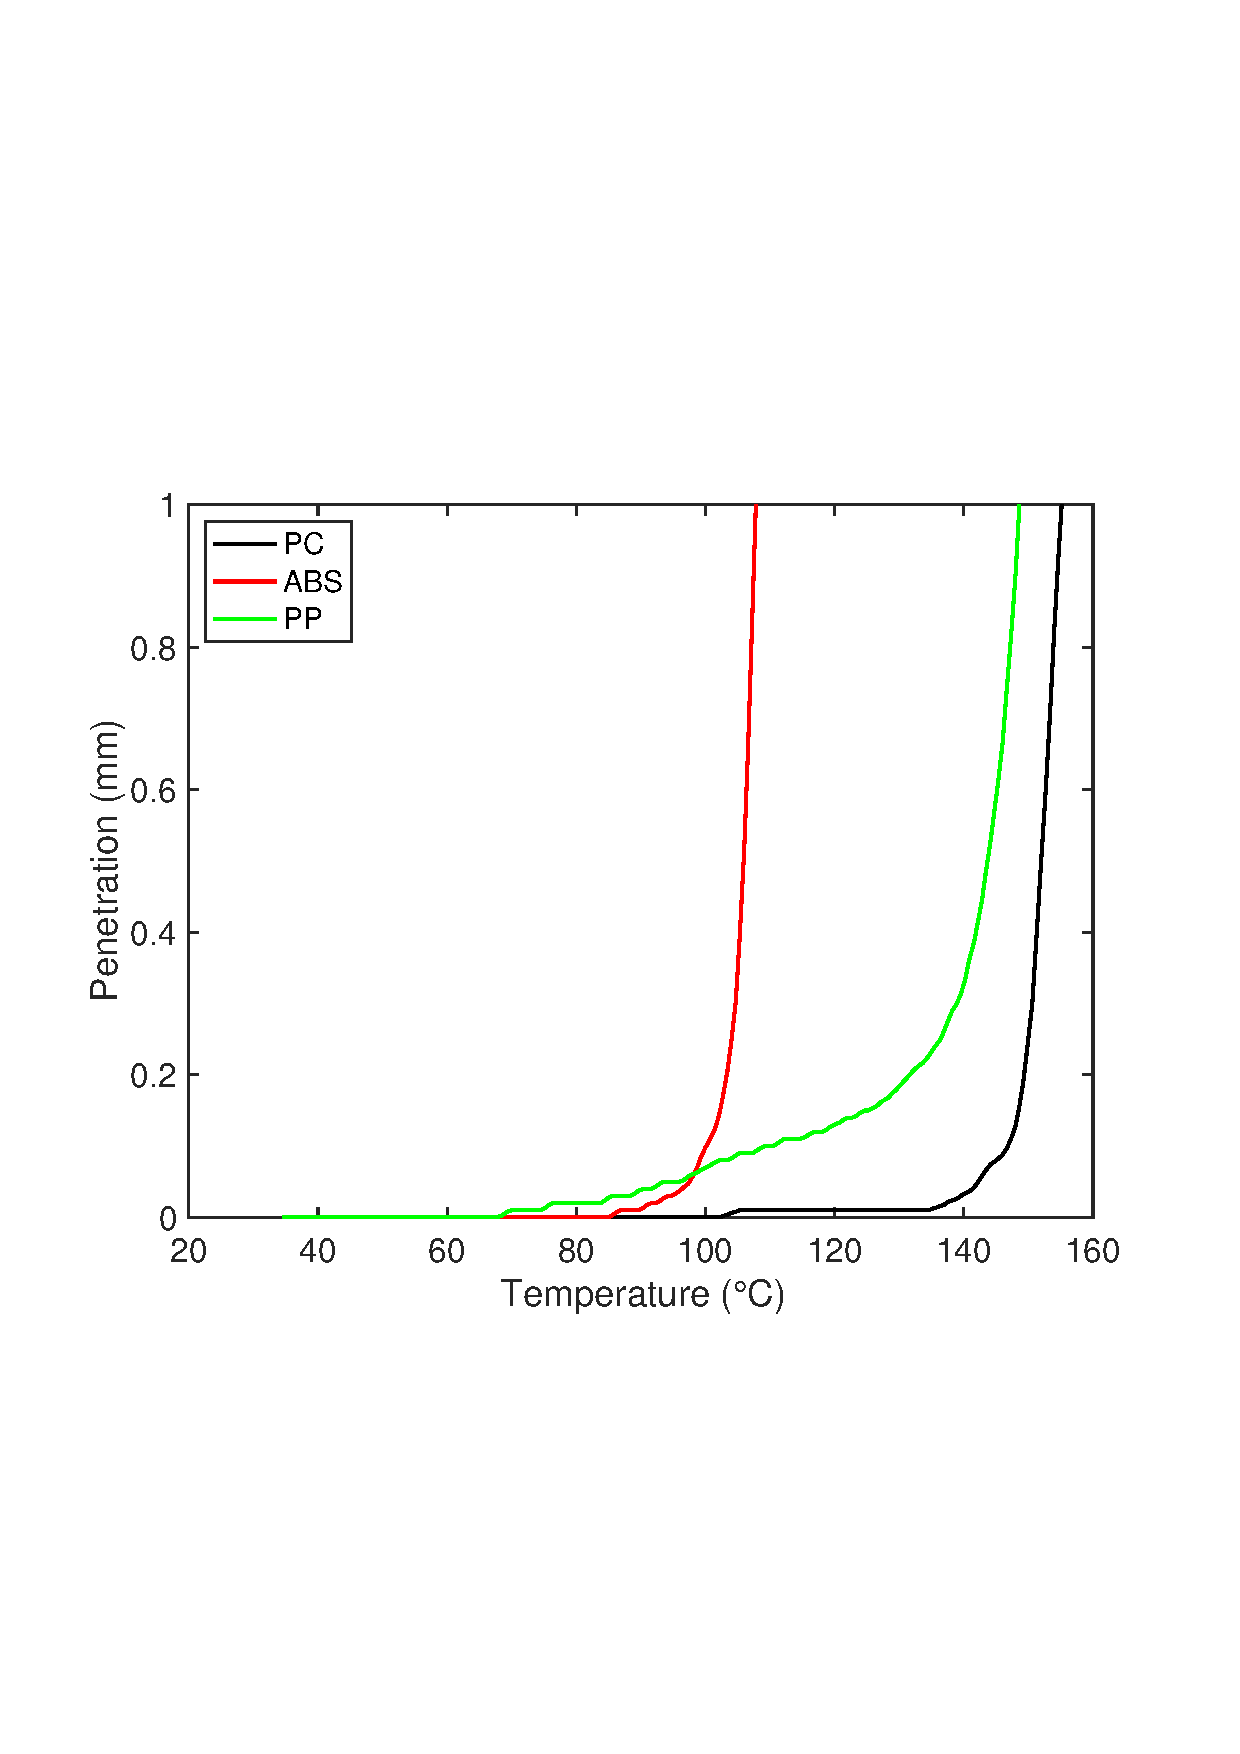
\includegraphics[scale=0.36]{vicat10}}\qquad
	\subfloat[][]
	{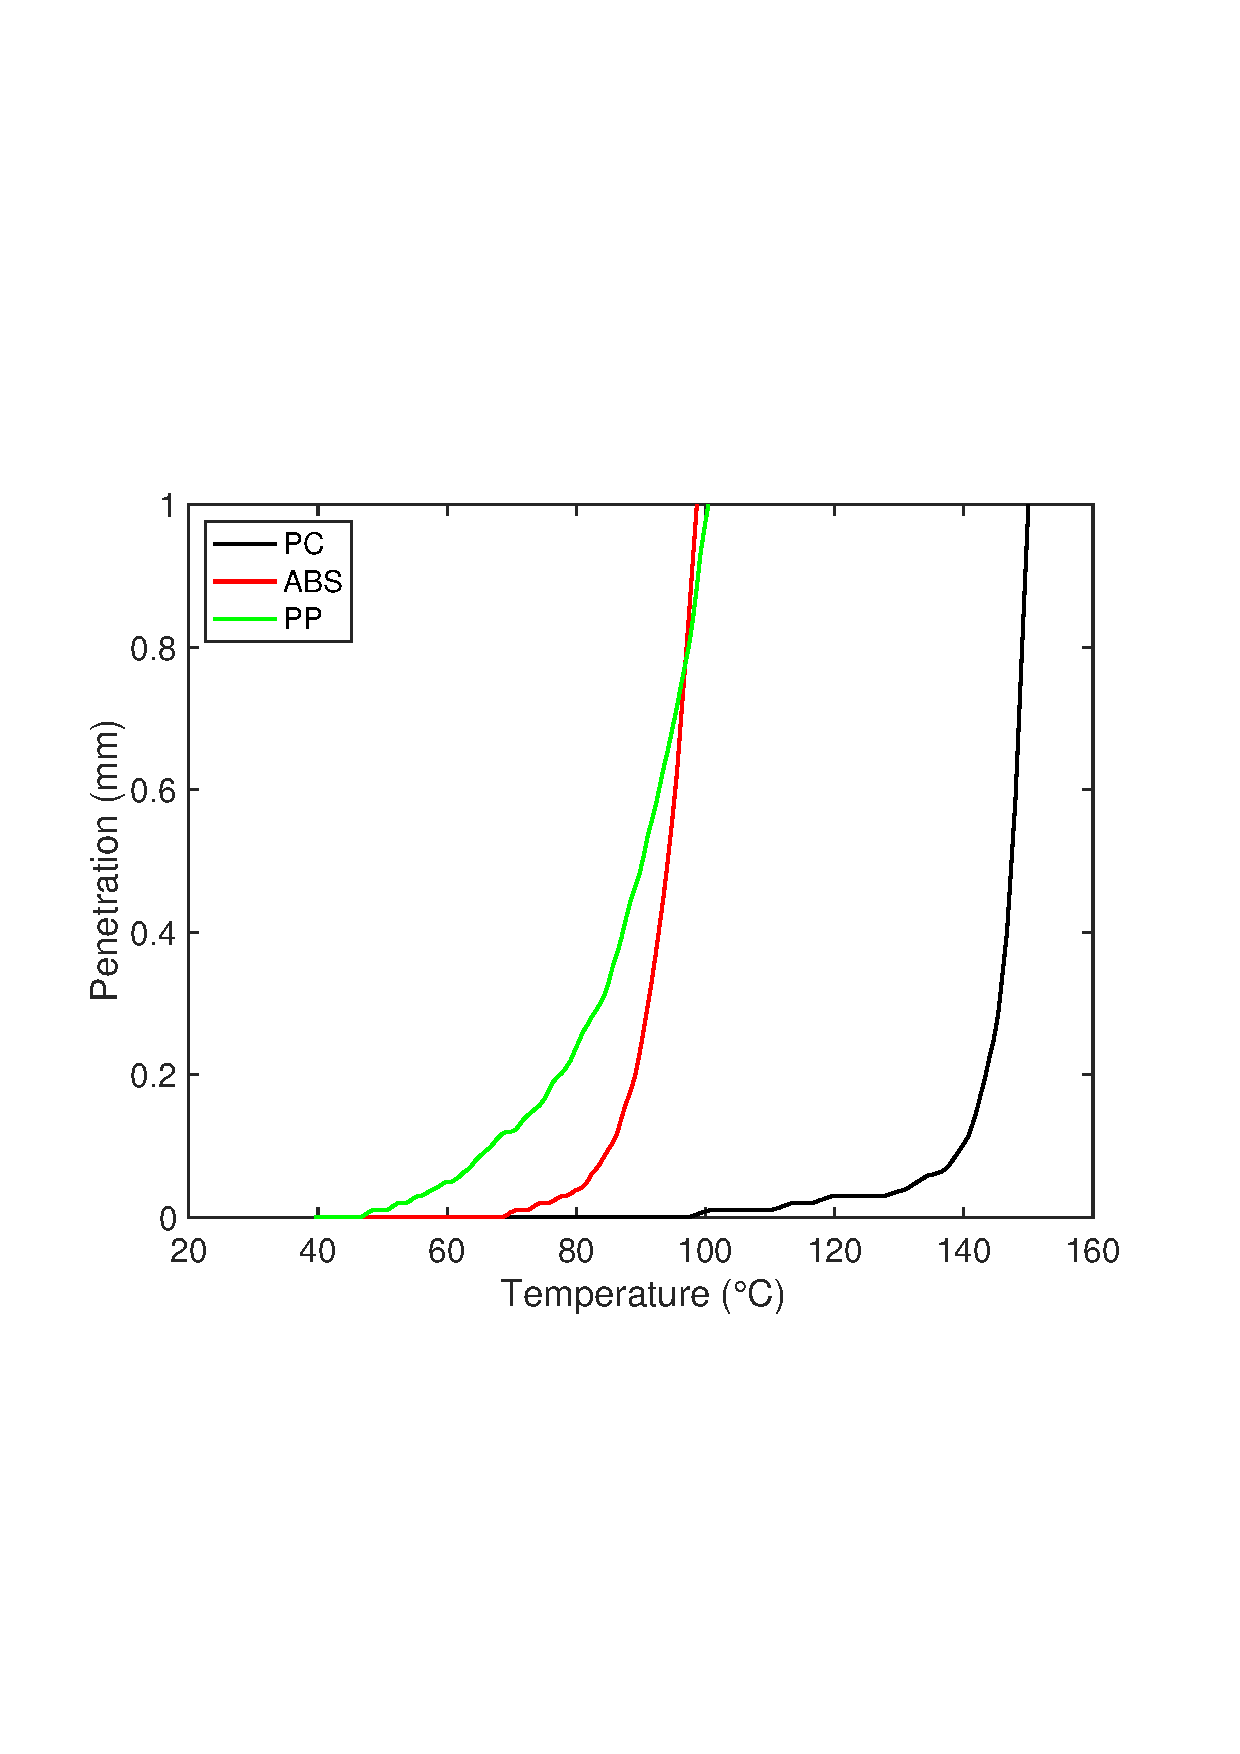
\includegraphics[scale=0.36]{vicat50}}\qquad
	\captionsetup{justification=centering}
	\caption{Vicat curves for a) $10$ N, b) $50$ N.}
	\label{fig:vicat}
\end{figure}

Analyzing the intersection between the curves and the penetration of $1$ mm the following data (\ref{tab:vicatt}) were obtained.

\begin{table}[htp]
	\centering
	$
	\begin{array}{cc}
	\toprule
	\textbf{Sample} & \mathbf{T_{Vicat}}\\
	\midrule
	\text{PC} & 1\\
	\text{ABS} & 1\\
	\text{PP} & 1\\
	\bottomrule
	\end{array}
	$
	\caption{Vicat temperatures}
	\label{tab:vicatt}
\end{table}

Since PC and ABS are amorphous polymers, their Vicat temperatures don't change substantionally with the load. This is due to the fact that the Vicat temperature corresponds to the glass transition temperature $T_{g}$ at which the polymer collapse under any load.\\
PP, instead, is a semicrystalline polymer, so its Vicat temperature varies considerably with the load. This can be explained by the presence of a rubbery amorphous phase that can be easily penetrated by the indent. The higher the load, the faster is the penetration.

\subsection{Limiting Oxygen Index}

The following table \ref{tab:loi} reports the main results obtained by this test.
\begin{table}[htp]
	\centering
	$
	\begin{array}{ccccc}
	\toprule
	\textbf{Sample} & \textbf{Oxygen ($\%$)} & \textbf{Flame} & \textbf{Smoke} & \textbf{Behaviour} \\
	\midrule
	\textbf{PE} & 20 & \text{yellow} & \text{no} & \text{drips}\\
	\textbf{PP} & 22 & \text{yellow} & \text{no} & \text{drips}\\
	\textbf{PC} & 33 & \text{undefined} & \text{yes} & \text{burns}\\
	\textbf{ABS} & 20 & \text{yellow, powerful} & \text{yes, with soot} & \text{burns}\\
	\bottomrule
	\end{array}
	$
	\caption{LOI results}
	\label{tab:loi}
\end{table}

PC sample reacts with a higher amount of blowed oxygen, meaning that this polymer is less flammable than the others.\\
In figure \ref{fig:loisamples} it is possible to see the samples reimainings after treatment.

\begin{figure}[htp]
	\centering
	{\includegraphics[scale=0.25]{loisamples}}
	\captionsetup{justification=centering}
	\caption{LOI samples after treatment: 1) PE, 2) PP, 3) PC, 4) ABS.}
	\label{fig:loisamples}
\end{figure}


\end{document}